\begin{question}
\noindent In a digital art app, a designer creates a triangular icon $ABC$ on a coordinate grid, then rotates it $90^{\circ}$ clockwise about the point $(0,0)$ to produce triangle $A'B'C'$ for a UI animation.

\begin{center}
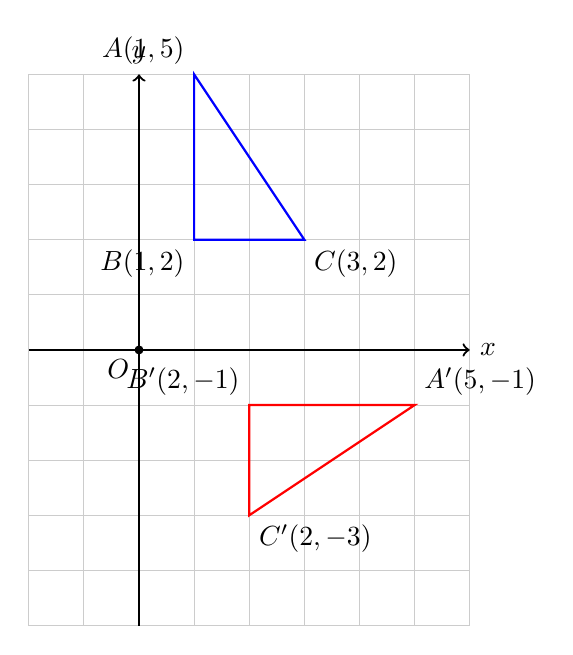
\begin{tikzpicture}[scale=0.7]
    \draw[thin, gray!40] (-2,-5) grid (6,5);
    \draw[thick,->] (-2,0) -- (6,0) node[right]{$x$};
    \draw[thick,->] (0,-5) -- (0,5) node[above]{$y$};

    % Triangle ABC
    \draw[thick, blue] (1,2) -- (1,5) -- (3,2) -- cycle;
    \node[above left] at (1,5) {$A(1,5)$};
    \node[below left] at (1,2) {$B(1,2)$};
    \node[below right] at (3,2) {$C(3,2)$};

    % Triangle A'B'C' (rotated 90 clockwise about origin: (x,y) -> (y,-x))
    \draw[thick, red] (5,-1) -- (2,-1) -- (2,-3) -- cycle;
    \node[above right] at (5,-1) {$A'(5,-1)$};
    \node[above left] at (2,-1) {$B'(2,-1)$};
    \node[below right] at (2,-3) {$C'(2,-3)$};

    \filldraw (0,0) circle (2pt) node[below left]{$O$};
\end{tikzpicture}
\end{center}

\noindent Triangle $ABC$ has vertices $A(1,5)$, $B(1,2)$ and $C(3,2)$.\\
Triangle $A'B'C'$ has vertices $A'(5,-1)$, $B'(2,-1)$ and $C'(2,-3)$.

\noindent Show that triangle $ABC$ is congruent to triangle $A'B'C'$ by comparing the lengths of all three corresponding sides.

\vspace{5cm}
\answermarks{3}
\end{question}
